

% Não é necessário alterar nada nesta primeira parte, esta primeira parte consiste na parte de configuração da linguagem e da formatação mais bruta do boletim epidemiológico %



%%%%%%%%%%%%%%%%%%%%%%%%%%%%%%%%%%%%%%%%%%%%%%%%%%%%%%%%%%%%%%%%%%%%%%%%%
% Este é um documento que servirá de modelo para os Boletins de         %
% Monitoramento de Eventos produzidos pela Sala de Situação de Saúde    %
% da Faculdade de Saúde - UnB                                           %
%%%%%%%%%%%%%%%%%%%%%%%%%%%%%%%%%%%%%%%%%%%%%%%%%%%%%%%%%%%%%%%%%%%%%%%%%


% Não é necessário alterar nada nesta primeira parte, esta primeira parte consiste na parte de configuração da linguagem e da formatação mais bruta do boletim de monitoramento de eventos de interesse à saúde %


% INÍCIO DA PRIMEIRA PARTE - NÃO ALTERAR NADA %



%Pacotes/bibliotecas utilizados:

\documentclass{article}
\usepackage[utf8]{inputenc}
\usepackage{graphicx}
\usepackage{eso-pic}
\usepackage{ifthen}
\usepackage{lipsum}
\usepackage{ragged2e}
\usepackage{xcolor}
\usepackage{multicol}
\usepackage{mwe}
\usepackage{wrapfig}
\setlength{\columnsep}{1cm} %%espaço entre as colunas de texto
%\def\columnseprulecolor{\color{blue}}
\def\columnseprulecolor{
\includegraphics{divisoria_vertical.png}}
\usepackage[a4paper, total={7.5in, 8in}]{geometry}
\usepackage[english]{babel}
\usepackage{fancyhdr}
\usepackage{ragged2e} %Para usar o comando que justifica o texto
\futurelet\TMPheaderrule\def\headrule{{
\includegraphics[width=\linewidth]{divisoria_horizontal.png}\TMPheaderrule}}
\usepackage[hidelinks]{hyperref}
\usepackage{url}
\hypersetup{
   colorlinks,
   %linkcolor={red!50!black},
   %citecolor={blue!50!black},
   urlcolor={blue!80!black}
}
\usepackage{scrextend}
\usepackage{moresize}
\usepackage{fontspec}
\setmainfont[BoldItalicFont=Myriad_Bold_Italic.ttf, BoldFont=MyriadPro-Bold.otf, ItalicFont=MyriadPro-It.otf]{MyriadPro-Regular.otf} %% Config. para usar fonte Myriad Pro, cujo arquivos estão na pasta do projeto

\newfontfamily{\calibrifont}[BoldItalicFont=CalibriBoldItalic.ttf, BoldFont=CalibriBold.ttf, ItalicFont=CalibriItalic.ttf]{Calibri.ttf}%Config para usar fonte Calibri cujo arquivos estão na pasta do projeto
\DeclareTextFontCommand{\calibri}{\calibrifont}%% permite usar calibri da forma: \calibri{texto em calibri}

\newcommand\addtopico[3]{ %%tipo função q ajusta posição do cabeçalho de tópico p quando for usar só chamar
\hspace*{-1in}
\begin{picture}(0,23)
\put(0,0){\includegraphics[width=100cm,height=1cm]{#1.png}}
\put(50,10){\textbf{\large #2}\includegraphics[width=0.8cm,height=0.5cm]{#3.png}}
\end{picture}
}

\newcommand\addtopicocespaco[4]{
\hspace*{-1in}
\begin{picture}(0,#4)
\put(0,0){\includegraphics[width=100cm,height=1cm]{#1.png}}
\put(50,10){\textbf{#2}\includegraphics[width=0.8cm,height=0.5cm]{#3.png}}
\end{picture}
}

\newcommand\addtopicopos[9]{
\hspace*{-1in}
\begin{picture}(#4,#5)
\put(#6,#7){\includegraphics[width=100cm,height=1cm]{#1.png}}
\put(#8,#9){\textbf{\large #2}\includegraphics[width=0.8cm,height=0.5cm]{#3.png}}
\end{picture}
}

\newcommand\addseccao[1]{
\hspace*{-1in}
\begin{picture}(0,45)
\put(26,0){\includegraphics[width=\paperwidth]{#1.png}}
\end{picture}
}

\newcommand\addtopicoref{
 \hspace*{-1in}
\begin{picture}(200,30)
\put(0,0){
\includegraphics[width=100cm,height=1.5cm]{fundo_topo_referencias.png}}
\put(50,10){\LARGE\textbf{REFERÊNCIAS}
\hspace*{0.3cm}

\includegraphics[width=1.5cm,height=1cm]{simboloreferencias.png}}
\end{picture}
}

\title{Modelo Boletim de Monitoramento de Eventos}

% FIM DA PRIMEIRA PARTE - NÃO ALTERAR NADA DA PRIMEIRA PARTE%



% ------ CAPA ------


% NÃO ALTERAR ESTA PARTE - configura a capa - NÃO ALTERAR ESTA PARTE%: 
\begin{document}
\pagestyle{empty}

% Este espaço serve para colocar a imagem desejada, a imagem irá aparecer justificado em harmonia com o texto colocado, para alterar a imagem basta inserir a imagem no canto superior esquerdo na aba "project", e assim irá abrir uma nova aba escrito "file", agora é necessário clicar na palavra "files" que está na cor cinza com um ícone de pasta ao lado, quando clicado no ícone "file" irá abrir uma janela com várias opções, aí é necessário selecionar a 9ª opção denominada "computer" que está no subitem uploade... computer, a escolha é de selecionar a imagem do computador e após a escolha é necessário clicar em enviar; após fazer isso é necessário observar qual o nome da imagem, e aí é necessário apenas acrescentar o nome da imagem nas chaves abaixo, conforme exemplo {capa_boletim_epidemiologico.png} é necessário colocar a extensão da imagem (no caso o .png), caso a imagem seja .jpg é necessário alterar o .png para o .jpg %
\AddToShipoutPictureBG{\ifthenelse{\value{page}>0}{}{\put(0,400){
\includegraphics[width=\paperwidth,height=16cm]{Capa.png}}}} 
\begin{frame}{}
\end{frame}
\vfill
\hspace*{-0.7in}%- NÃO ALTERAR ESTA PARTE%

\includegraphics[width=9in,height=0.7in]
{Semana_Epidemiologica.png} %-% Este espaço serve para colocar a imagem desejada, a imagem irá aparecer justificado em harmonia com o texto colocado, para alterar a imagem basta inserir a imagem no canto superior esquerdo na aba "project", e assim irá abrir uma nova aba escrito "file", agora é necessário clicar na palavra "files" que está na cor cinza com um ícone de pasta ao lado, quando clicado no ícone "file" irá abrir uma janela com várias opções, aí é necessário selecionar a 9ª opção denominada "computer" que está no subitem uploade... computer, a escolha é de selecionar a imagem do computador e após a escolha é necessário clicar em enviar; após fazer isso é necessário observar qual o nome da imagem, e aí é necessário apenas acrescentar o nome da imagem nas chaves abaixo, conforme exemplo {capa_boletim_epidemiologico.png} é necessário colocar a extensão da imagem (no caso o .png), caso a imagem seja .jpg é necessário alterar o .png para o .jpg %
\centering


\textbf{Ed. 11 - Maio de 2018}% Nesta linha é colocado o subtítulo que fica abaixo do título principal da página, para alterar é necessário trocar a frase dentro da chaves na cor preta pela frase desejada

\begin{multicols}{2}

\centering\large{EVENTOS NACIONAIS} %Esta linha é o título da primeira divisão da capa, para alterar é necessário trocar a frase na cor preta dentro da chaves para a frase desejada

\justifying
\vskip 0.2cm

\includegraphics[width=0.8cm,height=0.5cm]{Monitoramento.png}\put(0,5.5){\large Febre Amarela (Pág. 01)}\\ %Esta linha foi especificado qual o nome do tópico dos eventos nacionais e em qual página vai estar, para alterar basta trocar o nome na última chaves da linha para o nome desejado


\includegraphics[width=0.8cm,height=0.5cm]{Monitoramento.png}\put(0,5.5){\large Sarampo (Pág. 02)}\\  %Esta linha foi especificado qual o nome do tópico dos eventos nacionais e em qual página vai estar, para alterar basta trocar o nome na última chaves da linha para o nome desejado


\includegraphics[width=0.8cm,height=0.5cm]{Alerta.png}\put(0,5.5){\large Influenza (Pág. 03)}\\  %Esta linha foi especificado qual o nome do tópico dos eventos nacionais e em qual página vai estar, para alterar basta trocar o nome na última chaves da linha para o nome desejado


\includegraphics[width=0.8cm,height=0.5cm]{Monitoramento.png}\put(0,5.5){\large Conjuntivite no Brasil (Pág. 03)}\\ %Esta linha foi especificado qual o nome do tópico dos eventos nacionais e em qual página vai estar, para alterar basta trocar o nome na última chaves da linha para o nome desejado



\includegraphics[width=0.8cm,height=0.5cm]{Monitoramento.png}\put(0,5.5){\large Toxoplasmose no Sul do Brasil (Pág. 04)}\\ %Esta linha foi especificado qual o nome do tópico dos eventos nacionais e em qual página vai estar, para alterar basta trocar o nome na última chaves da linha para o nome desejado

\columnbreak 

\centering\large{EVENTOS INTERNACIONAIS} %Esta linha é o título da primeira divisão da capa, para alterar é necessário trocar a frase na cor preta dentro da chaves para a frase desejado

\justifying
\vskip 0.2cm

\includegraphics[width=0.8cm,height=0.5cm]{Monitoramento.png}\put(0,5.5){\large Guillain-Barré no Peru (Pág. 05)}\\  %Esta linha foi especificado qual o nome do tópico dos eventos internacionais e em qual página vai estar, para alterar basta trocar o nome na última chaves da linha para o nome desejado


\includegraphics[width=0.8cm,height=0.5cm]{Monitoramento.png}\put(0,5.5){\large Ebola na República Democrática do Congo (Pág. 05)}\\ %Esta linha foi especificado qual o nome do tópico dos eventos internacionais e em qual página vai estar, para alterar basta trocar o nome na última chaves da linha para o nome desejado

\end{multicols}

%Esta parte é utilizada para colocar a última linha da capa, parar alterar é necessário alterar apenas o que está em preto na última chaves de cada linha
\centering
{
\includegraphics[width=0.8cm,height=0.5cm]{Alerta.png} Eventos em alerta}\quad %se for alterar, alterar apenas o que está na última chaves
{
\includegraphics[width=0.8cm,height=0.5cm]{Monitoramento.png} Eventos em monitoramento}\quad %se for alterar, alterar apenas o que está na última chaves
{
\includegraphics[width=0.8cm,height=0.5cm]{Encerramento.png} Eventos em encerramento} %se for alterar, alterar apenas o que está na última chaves

%Esta linha é para colocar o plano de fundo nas páginas com exceção da primeira, para alterar basta inserir a imagem no canto superior esquerdo na aba "project", e assim irá abrir uma nova aba escrito "file", agora é necessário clicar na palavra "files" que está na cor cinza com um ícone de pasta ao lado, quando clicado no ícone "file" irá abrir uma janela com várias opções, aí é necessário selecionar a 9ª opção denominada "computer" que está no subitem uploade... computer, a escolha é de selecionar a imagem do computador e após a escolha é necessário clicar em enviar; após fazer isso é necessário observar qual o nome da imagem, e aí é necessário apenas acrescentar o nome da imagem nas chaves abaixo, conforme exemplo {fundo_paginas.png} é necessário colocar a extensão da imagem (no caso o .png), caso a imagem seja .jpg é necessário alterar o .png para o .jpg %
\AddToShipoutPictureBG{\ifthenelse{\value{page}<1}{}{
\includegraphics[width=\paperwidth,height=\paperheight]{fundo_paginas.pdf}}}
\setcounter{page}{0}

% Grupos de tamanho de letra: tiny, scriptsize, footnotesize, small, normalsize, large, Large, huge, Huge. 

\newpage
\justifying
\pagestyle{fancy}
\fancyhf{}
\rhead{\thepage}
\lhead{BOLETIM DE MONITORAMENTO DE EVENTOS DE INTERESSE À SAÚDE | SEMANA 19} %Esta linha serve para colocar o título superior da página, para alterar basta trocar a frase que está na cor preta nas chaves pela frase desejada

\justifying
\addseccao{Eventos_Nacionais} %Esta linha da o título principal da pagina, para alterar basta trocar a frase que está na cor preta nas chaves pela frase desejada


%adiciona tópicos na página%
\addtopico{Tarja_nacional}{FEBRE AMARELA}{Monitoramento} %Esta linha serve para adcionar o tópico junto com o losango sem necessitar de formatação, neste caso específico para chamar o da febre amarela é necessário apenas escrever "monitoramento" dentro das chaves, e para alterar a frase "febre amarela" basta trocar a frase que está na cor preta nas chaves pela frase desejada 

\begin{wrapfigure}{R}{0.5\textwidth}
\centering
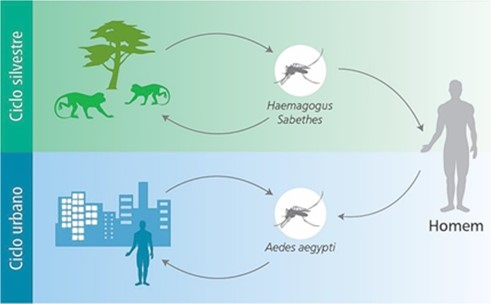
\includegraphics[width=.5\textwidth]{img_altera_1.jpg}
\end{wrapfigure}

\par


{\large %%%Está linha é utilizada para aumentar a fonte pois a fonte padrão do latex é menor, não é necessário alterar essa parte,a menos que seja necessário alterar tamanho da fonte. Neste caso, \large pode ser alterado para uma dessas opções da menor para maior: \tiny, \scriptsize, \footnotesize, \small, \normalsize, \arge, \Large, \huge, \Huge .

 % Esta parte é utilizada para colocar o texto do tópico, para alterar basta alterar o que está escrito na cor preta dentro das chaves
    
	A febre amarela é uma doença infecciosa febril aguda, imunoprevenível, causada por um vírus transmitido por mosquitos vetores, e possui dois ciclos de transmissão: silvestre (quando há transmissão em área rural ou de floresta) e urbano. O vírus é transmitido pela picada dos mosquitos transmissores infectados e não há transmissão direta de pessoa a pessoa. A doença tem importância epidemiológica por sua gravidade clínica e potencial de disseminação em áreas urbanas infestadas pelo mosquito \textit{Aedes aegypti}.\textsuperscript{1}

\justifying


\includegraphics[width=\linewidth]{divisoria_horizontal.png} % Este espaço serve para colocar a divisória horizontal para melhor formatação do boletim

\justifying

 % Esta parte é utilizada para continuação do texto do tópico, para alterar basta alterar o que está escrito na cor preta dentro das chaves
 
	Entre julho de 2017 e 8 de maio de 2018, o Brasil registrou 409 mortes por febre amarela, informa o último boletim epidemiológico divulgado pelo Ministério da Saúde.No boletim anterior, que contabilizou dados até o 2 de maio, o país registrava 394 mortes. Em todo o período, a pasta confirmou 1261 infecções. O ministério investiga ainda 1301 casos. Em relação aos dados anteriores, a pasta registra mais 15 mortes. Há também mais 4 casos confirmados em sete dias.\textsuperscript{2}

	A Organização Mundial da Saúde (OMS) passou a recomendar a vacinação contra febre amarela para todos os viajantes internacionais que visitem qualquer área dos estados da região Sul do Brasil (Paraná, Santa Catarina e Rio Grande do Sul). Até então, algumas partes desses estados não eram consideradas de risco para a doença.\textsuperscript{3}

} %%Chave que finaliza o bloco de texto com tamanho \large

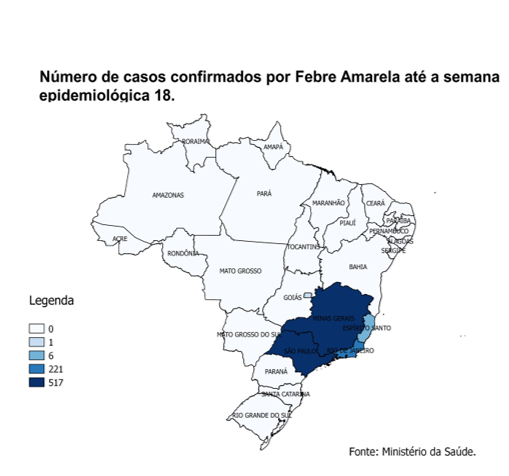
\includegraphics[width=.4\textwidth]{img_altera_2.png}% Este espaço serve para colocar a imagem desejada, a imagem irá aparecer justificado em harmonia com o texto colocado, para alterar a imagem basta inserir a imagem no canto superior esquerdo na aba "project", e assim irá abrir uma nova aba escrito "file", agora é necessário clicar na palavra "files" que está na cor cinza com um ícone de pasta ao lado, quando clicado no ícone "file" irá abrir uma janela com várias opções, aí é necessário selecionar a 9ª opção denominada "computer" que está no subitem uploade... computer, a escolha é de selecionar a imagem do computador e após a escolha é necessário clicar em enviar; após fazer isso é necessário observar qual o nome da imagem, e aí é necessário apenas acrescentar o nome da imagem nas chaves abaixo, conforme exemplo {capa_boletim_epidemiologico.png} é necessário colocar a extensão da imagem (no caso o .png), caso a imagem seja .jpg é necessário alterar o .png para o .jpg %
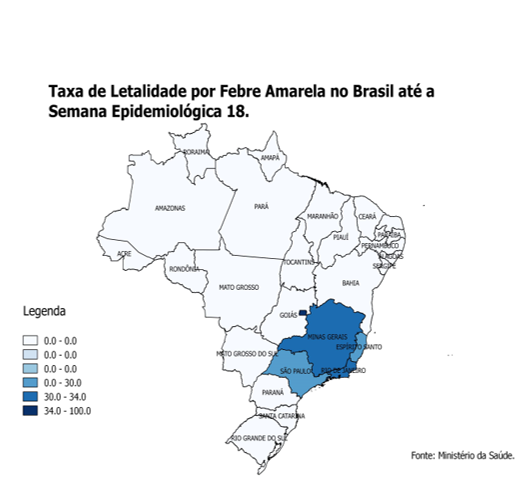
\includegraphics[width=.4\textwidth]{img_altera_3.png}% Este espaço serve para colocar a imagem desejada, a imagem irá aparecer justificado em harmonia com o texto colocado, para alterar a imagem basta inserir a imagem no canto superior esquerdo na aba "project", e assim irá abrir uma nova aba escrito "file", agora é necessário clicar na palavra "files" que está na cor cinza com um ícone de pasta ao lado, quando clicado no ícone "file" irá abrir uma janela com várias opções, aí é necessário selecionar a 9ª opção denominada "computer" que está no subitem uploade... computer, a escolha é de selecionar a imagem do computador e após a escolha é necessário clicar em enviar; após fazer isso é necessário observar qual o nome da imagem, e aí é necessário apenas acrescentar o nome da imagem nas chaves abaixo, conforme exemplo {capa_boletim_epidemiologico.png} é necessário colocar a extensão da imagem (no caso o .png), caso a imagem seja .jpg é necessário alterar o .png para o .jpg %




\addtopico{Tarja_nacional}{SARAMPO}{Alerta} %Esta linha serve para adcionar o tópico junto com o losango sem necessitar de formatação, neste caso específico para chamar o do sarampo é necessário apenas escrever "Alerta" dentro das chaves, e para alterar a frase "sarampo" basta trocar a frase que está na cor preta nas chaves pela frase desejada 

{\large %%%Está linha é utilizada para aumentar a fonte pois a fonte padrão do latex é menor, não é necessário alterar essa parte,a menos que seja necessário alterar tamanho da fonte. Neste caso, \large pode ser alterado para uma dessas opções da menor para maior: \tiny, \scriptsize, \footnotesize, \small, \normalsize, \arge, \Large, \huge, \Huge .

% Esta parte é utilizada para colocar o texto do tópico, para alterar basta alterar o que está escrito na cor preta dentro das chaves

	O Sarampo é uma doença infecciosa aguda, de natureza viral, grave, transmissível e extremamente contagiosa, muito comum na infância. A presença do vírus no sangue provoca uma vasculite generalizada, responsável pelo aparecimento das diversas manifestações clínicas, inclusive pelas perdas consideráveis de eletrólitos e proteínas. Isso resulta no quadro espoliante característico da infecção. Além disso, as complicações infecciosas contribuem para a gravidade do Sarampo, particularmente em crianças desnutridas e menores de um ano de idade. A doença é de distribuição universal e apresenta variação sazonal. Nos climas temperados, observa-se o aumento da incidência no período compreendido entre o final do inverno e o início da primavera. Nos climas tropicais, a transmissão parece au1mentar depois da estação chuvosa. O comportamento endêmico do Sarampo varia, de um local para outro, e depende basicamente da relação entre o grau de imunidade e a suscetibilidade da população, além da circulação do vírus na área.\textsuperscript{4}


\includegraphics[width=\linewidth]{divisoria_horizontal.png}  %Este espaço serve para colocar a divisória horizontal para melhor formatação do boletim

\begin{wrapfigure}{R}{0.3\textwidth}
\centering
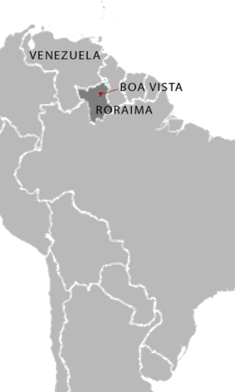
\includegraphics[width=.2\textwidth]{img_altera_4.png}% Este espaço serve para colocar a imagem desejada, a imagem irá aparecer justificado em harmonia com o texto colocado, para alterar a imagem basta inserir a imagem no canto superior esquerdo na aba "project", e assim irá abrir uma nova aba escrito "file", agora é necessário clicar na palavra "files" que está na cor cinza com um ícone de pasta ao lado, quando clicado no ícone "file" irá abrir uma janela com várias opções, aí é necessário selecionar a 9ª opção denominada "computer" que está no subitem uploade... computer, a escolha é de selecionar a imagem do computador e após a escolha é necessário clicar em enviar; após fazer isso é necessário observar qual o nome da imagem, e aí é necessário apenas acrescentar o nome da imagem nas chaves abaixo, conforme exemplo {capa_boletim_epidemiologico.png} é necessário colocar a extensão da imagem (no caso o .png), caso a imagem seja .jpg é necessário alterar o .png para o .jpg %
\end{wrapfigure}

\par

\justifying
 % Esta parte é utilizada para continuação do texto do tópico, para alterar basta alterar o que está escrito na cor preta dentro das chaves
	Segundo a Secretaria Estadual de Saúde de Roraima subiu para 83 o número de casos confirmados de sarampo. Deste total, 62 foram registrados somente em Boa Vista, sendo 57 deles em venezuelanos.\textsuperscript{5}

	O ministério da Saúde informou que de janeiro até o dia 30 de abril de 2018 o país registrou duas mortes por sarampo, ambas no estado de Roraima, onde evolução para óbito ocorreu nesses casos porque havia comorbidades nesses pacientes.\textsuperscript{6}

	A organização Mundial de Saúde emitiu um alerta sobre sarampo nas América e exortou países a reforçarem a vacinação. Ao todo foram registrados 1115 casos na região. Superando o número registrado no ano anterior.\textsuperscript{7}
    
} %%Chave que finaliza o bloco de texto com tamanho \large

    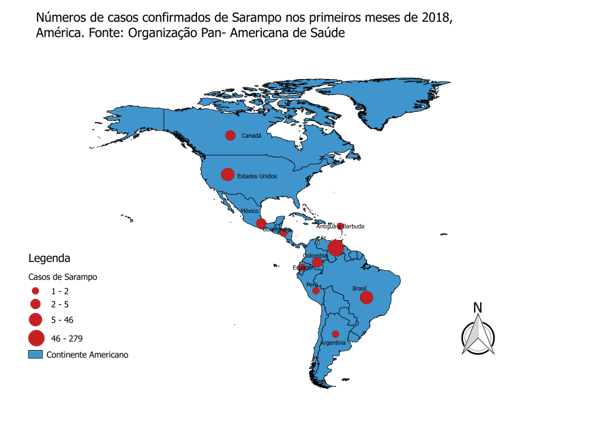
\includegraphics[width=.6\textwidth]{img_altera_5.png}% Este espaço serve para colocar a imagem desejada, a imagem irá aparecer justificado em harmonia com o texto colocado, para alterar a imagem basta inserir a imagem no canto superior esquerdo na aba "project", e assim irá abrir uma nova aba escrito "file", agora é necessário clicar na palavra "files" que está na cor cinza com um ícone de pasta ao lado, quando clicado no ícone "file" irá abrir uma janela com várias opções, aí é necessário selecionar a 9ª opção denominada "computer" que está no subitem uploade... computer, a escolha é de selecionar a imagem do computador e após a escolha é necessário clicar em enviar; após fazer isso é necessário observar qual o nome da imagem, e aí é necessário apenas acrescentar o nome da imagem nas chaves abaixo, conforme exemplo {capa_boletim_epidemiologico.png} é necessário colocar a extensão da imagem (no caso o .png), caso a imagem seja .jpg é necessário alterar o .png para o .jpg %
    
    
    
    

\addtopico{Tarja_nacional}{INFLUENZA NO BRASIL}{Alerta} %Esta linha serve para adcionar o tópico junto com o losango sem necessitar de formatação, neste caso específico para chamar o do influenza é necessário apenas escrever "Alerta" dentro das chaves, e para alterar a frase "sarampo" basta trocar a frase que está na cor preta nas chaves pela frase desejada


\includegraphics[width=\linewidth]{divisoria_horizontal.png} %Este espaço serve para colocar a divisória horizontal para melhor formatação do boletim

{\large %%%Está linha é utilizada para aumentar a fonte pois a fonte padrão do latex é menor, não é necessário alterar essa parte,a menos que seja necessário alterar tamanho da fonte. Neste caso, \large pode ser alterado para uma dessas opções da menor para maior: \tiny, \scriptsize, \footnotesize, \small, \normalsize, \arge, \Large, \huge, \Huge .

% Esta parte é utilizada para colocar o texto do tópico, para alterar basta alterar o que está escrito na cor preta dentro das chaves

A influenza ou gripe é uma infecção aguda do sistema respiratório, ocasionada pelo vírus influenza, com elevado potencial de transmissão. Inicia-se com febre, dor muscular, e tosse seca. Em geral, tem evolução por período limitado, em geral de um a quatro dias, mas pode se apresentar forma grave.\textsuperscript{8}


\includegraphics[width=\linewidth]{divisoria_horizontal.png} %Este espaço serve para colocar a divisória horizontal para melhor formatação do boletim

% Esta parte é utilizada para continuação do texto do tópico, para alterar basta alterar o que está escrito na cor preta dentro das chaves

	Dois novos casos de H1N1 foram confirmados pela Secretaria de Saúde noinforme epidemiológico divulgado nesta segunda-feira(7). De janeiro até o final de abril, 17 pessoas foram contaminadas pelo vírus H1N1 no DF euma morreu.De acordo com a secretaria, menos de 40\% do público alvo recebeu a vacina contra a gripe até agora.\textsuperscript{9}

	A terceira morte de um paciente com o vírus da gripe H1N1 foi confirmada nesta terça-feira (8) pela Secretaria Estadual de Saúde. De acordo com o último boletim epidemiológico divulgado pelo órgão, exames laboratoriais confirmaram a presença do vírus em três pacientes de síndrome respiratória aguda grave que morreram em 2018.\textsuperscript{10}
    
	A Fundação Municipal de Saúde (FMS) atualizou os dados relacionados ao número de casos de gripe H1N1 em Teresina. Atualmente são 32 o número de registros confirmados pela fundação, com uma morte registrada resultante da infecção do vírus da Influenza A. Outras duas mortes estão sob investigação. O Levantamento foi atualizado na tarde desta terça-feira (8).\textsuperscript{11}
    
	Um homem, de 27 anos, morreu com a gripe H1N1 em Santa Fé do Sul (SP) nesta segunda-feira (7), segundo a Secretaria de Saúde da cidade.\textsuperscript{12}\\
\\
\par
} %%Chave que finaliza o bloco de texto com tamanho \large





\addtopico{Tarja_nacional}{CONJUNTIVITE NO BRASIL}{Monitoramento} %Esta linha serve para adcionar o tópico junto com o losango sem necessitar de formatação, neste caso específico para chamar o da conjuntivite é necessário apenas escrever "Monitoramento" dentro das chaves, e para alterar a frase "Conjuntivite no Brasil" basta trocar a frase que está na cor preta nas chaves pela frase desejada

\begin{wrapfigure}{L}{0.3\textwidth} %this figure will be at the right
    \centering
    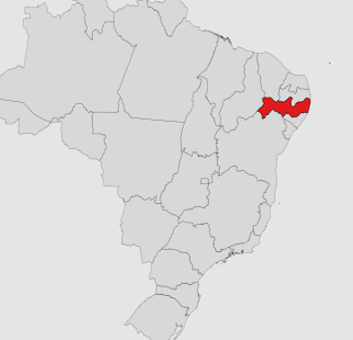
\includegraphics[width=0.3\textwidth]{img_altera_6.png} % Este espaço serve para colocar a imagem desejada, a imagem irá aparecer justificado em harmonia com o texto colocado, para alterar a imagem basta inserir a imagem no canto superior esquerdo na aba "project", e assim irá abrir uma nova aba escrito "file", agora é necessário clicar na palavra "files" que está na cor cinza com um ícone de pasta ao lado, quando clicado no ícone "file" irá abrir uma janela com várias opções, aí é necessário selecionar a 9ª opção denominada "computer" que está no subitem uploade... computer, a escolha é de selecionar a imagem do computador e após a escolha é necessário clicar em enviar; após fazer isso é necessário observar qual o nome da imagem, e aí é necessário apenas acrescentar o nome da imagem nas chaves abaixo, conforme exemplo {capa_boletim_epidemiologico.png} é necessário colocar a extensão da imagem (no caso o .png), caso a imagem seja .jpg é necessário alterar o .png para o .jpg %
\end{wrapfigure}
\noindent
\\
{\large %Está linha é utilizada para aumentar a fonte pois a fonte padrão do latex é menor, não é necessário alterar essa parte,a menos que seja necessário alterar tamanho da fonte. Neste caso, \large pode ser alterado para uma dessas opções da menor para maior: \tiny, \scriptsize, \footnotesize, \small, \normalsize, \arge, \Large, \huge, \Huge .

% Esta parte é utilizada para colocar o texto do tópico, para alterar basta alterar o que está escrito na cor preta dentro das chaves

	Conjuntivite é a inflamação da conjuntiva, membrana transparente e fina que reveste a parte da frente do globo ocular (o branco dos olhos) e o interior das pálpebras. Em geral, ataca os dois olhos, pode durar de uma semana a 15 dias e não costuma deixar sequelas.\textsuperscript{13}  } %%Chave que finaliza o bloco de texto com tamanho \large    
\\

\includegraphics[width=\linewidth]{divisoria_horizontal.png} %Este espaço serve para colocar a divisória horizontal para melhor formatação do boletim
\\
	{\large %%Está linha é utilizada para aumentar a fonte pois a fonte padrão do latex é menor, não é necessário alterar essa parte,a menos que seja necessário alterar tamanho da fonte. Neste caso, \large pode ser alterado para uma dessas opções da menor para maior: \tiny, \scriptsize, \footnotesize, \small, \normalsize, \arge, \Large, \huge, \Huge .
    
    % Esta parte é utilizada para continuação do texto do tópico, para alterar basta alterar o que está escrito na cor preta dentro das chaves
    
    A Fundação Altino Ventura (FAV), hospital de referência que oferece atendimento gratuito no Recife, recebeu, no mês de abril, 15 mil pessoas com conjuntivite. Esse número é 22 vezes maior que o registrado em abril de 2017, quando foram realizados 691 atendimentos.\textsuperscript{14} } %Chave que finaliza o bloco de texto com tamanho \large
\\
\\
\\
\\
\\
\\
\\
\\
\\
\\
\\

\addtopico{Tarja_nacional}{TOXOPLASMOSE NO SUL DO BRASIL}{Alerta}  %Esta linha serve para adcionar o tópico junto com o losango sem necessitar de formatação, neste caso específico para chamar o da toxoplasmose é necessário apenas escrever "Alerta" dentro das chaves, e para alterar a frase "Toxoplasmose no sul do Brasil" basta trocar a frase que está na cor preta nas chaves pela frase desejada


  {\large %%Está linha é utilizada para aumentar a fonte pois a fonte padrão do latex é menor, não é necessário alterar essa parte,a menos que seja necessário alterar tamanho da fonte. Neste caso, \large pode ser alterado para uma dessas opções da menor para maior: \tiny, \scriptsize, \footnotesize, \small, \normalsize, \arge, \Large, \huge, \Huge .
  
  % Esta parte é utilizada para colocar o texto do tópico, para alterar basta alterar o que está escrito na cor preta dentro das chaves

    A toxoplasmose é uma doença infecciosa causada por um protozoário chamado \textit{Toxoplasma gondii}, que é encontrado na natureza e pode causar infecção em grande número de mamíferos e pássaros no mundo todo. A doença pode ocorrer pela ingestão de oocistos provenientes do solo, areia, latas de lixo contaminadas pelasfezes de gatos infectados, ingestão de carne crua e malcozida infectada com cistos ou por intermédio de infecção transplancentária, ocorrendo em 40\% dos fetos de mães que adquiriam a infecção durante a gravidez.\textsuperscript{15}


\includegraphics[width=\linewidth]{divisoria_horizontal.png} %Este espaço serve para colocar a divisória horizontal para melhor formatação do boletim

 % Esta parte é utilizada para continuação do texto do tópico, para alterar basta alterar o que está escrito na cor preta dentro das chaves
A Secretaria Estadual da Saúde de Santa Maria, consideram o surto de toxoplasmose o maior já enfrentado no Rio Grande do Sul. O número de infectados cresceu 70\% em uma semana.\textsuperscript{16}

O número de casos de casos de toxoplasmose chegou a 2018. Foram notificados 729 casos na cidade, sendo que 617 foram considerados suspeitos e os outros 175 ainda aguardam classificação. Destes, 70 foram descartados, mas 319 estão sob investigação.\textsuperscript{17}

Enquanto não se descobre a causa da contaminação, novas medidas foram anunciadas para a prevenção da disseminação da doença. A criação de um ambulatório específico para exames oftalmológicos de pacientes suspeitos ou portadores do agravo. O credenciamento de laboratórios de Santa Maria para a realização de exames que possam fazer a contraprova da toxoplasmose. Além da busca de mais medicamentos para tratar a doença junto ao Ministério da Saúde.\textsuperscript{18}

} %%Chave que finaliza o bloco de texto com tamanho \large

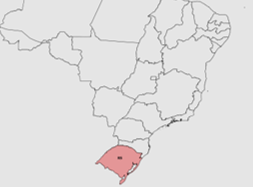
\includegraphics[width=.3\textwidth]{img_altera_8.png}  % Este espaço serve para colocar a imagem desejada, a imagem irá aparecer justificado em harmonia com o texto colocado, para alterar a imagem basta inserir a imagem no canto superior esquerdo na aba "project", e assim irá abrir uma nova aba escrito "file", agora é necessário clicar na palavra "files" que está na cor cinza com um ícone de pasta ao lado, quando clicado no ícone "file" irá abrir uma janela com várias opções, aí é necessário selecionar a 9ª opção denominada "computer" que está no subitem uploade... computer, a escolha é de selecionar a imagem do computador e após a escolha é necessário clicar em enviar; após fazer isso é necessário observar qual o nome da imagem, e aí é necessário apenas acrescentar o nome da imagem nas chaves abaixo, conforme exemplo {capa_boletim_epidemiologico.png} é necessário colocar a extensão da imagem (no caso o .png), caso a imagem seja .jpg é necessário alterar o .png para o .jpg %
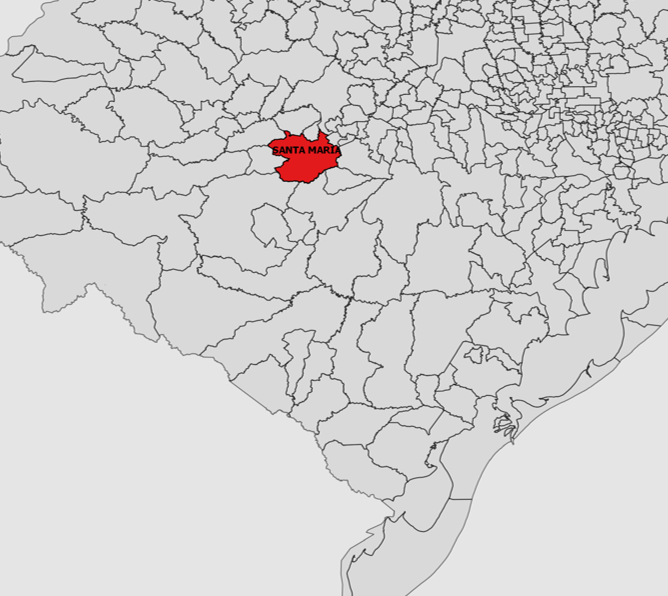
\includegraphics[width=.6\textwidth]{img_altera_7.png}  % Este espaço serve para colocar a imagem desejada, a imagem irá aparecer justificado em harmonia com o texto colocado, para alterar a imagem basta inserir a imagem no canto superior esquerdo na aba "project", e assim irá abrir uma nova aba escrito "file", agora é necessário clicar na palavra "files" que está na cor cinza com um ícone de pasta ao lado, quando clicado no ícone "file" irá abrir uma janela com várias opções, aí é necessário selecionar a 9ª opção denominada "computer" que está no subitem uploade... computer, a escolha é de selecionar a imagem do computador e após a escolha é necessário clicar em enviar; após fazer isso é necessário observar qual o nome da imagem, e aí é necessário apenas acrescentar o nome da imagem nas chaves abaixo, conforme exemplo {capa_boletim_epidemiologico.png} é necessário colocar a extensão da imagem (no caso o .png), caso a imagem seja .jpg é necessário alterar o .png para o .jpg %
\newpage


\addseccao{Eventos_Internacionais}  %Esta linha da o título principal da pagina, para alterar basta trocar a frase que está na cor preta nas chaves pela frase desejada

%adiciona topicos em posicoes específicas da página%
%(0,27) => posição do topico%
%(0,20) => posição da imagem de fundo%
%(50,30) => posição do título do tópico%
\addtopicopos{Tarja_intern}{GUILLAIN-BARRÉ NO PERU}{Alerta}{0}{27}{0}{20}{50}{30} %Esta linha serve para adcionar o tópico junto com o losango sem necessitar de formatação, neste caso específico para chamar o da guillain é necessário apenas escrever "Alerta" dentro das chaves, e para alterar a frase "GUILLAIN-BARRÉ NO PERU" basta trocar a frase que está na cor preta nas chaves pela frase desejada

{\large %%Está linha é utilizada para aumentar a fonte pois a fonte padrão do latex é menor, não é necessário alterar essa parte,a menos que seja necessário alterar tamanho da fonte. Neste caso, \large pode ser alterado para uma dessas opções da menor para maior: \tiny, \scriptsize, \footnotesize, \small, \normalsize, \arge, \Large, \huge, \Huge .


% Esta parte é utilizada para colocar o texto do tópico, para alterar basta alterar o que está escrito na cor preta dentro das chaves

	A Síndrome de Guillain-Barré (SGB), também conhecida por Polirradiculoneurite Aguda, é uma rara doença neurológica, de origem autoimune, provocada por diversos fatores, entre eles infecções virais e bacterianas, cuja progressão se dá por uma sensação de parestesias nas extremidades distais dos membros inferiores e superiores, com dor neuropática se estabelecendo em metade dos casos.\textsuperscript{19}
   
   
\includegraphics[width=\linewidth]{divisoria_horizontal.png} %Este espaço serve para colocar a divisória horizontal para melhor formatação do boletim
   
    % Esta parte é utilizada para continuação do texto do tópico, para alterar basta alterar o que está escrito na cor preta dentro das chaves
    
   O Ministério da Saúde do Peru declarou um alerta epidemiológico nacional para contar o que parece ser um surto da síndrome de Guillain-Barré, que está associada ao vírus Zika. Autoridades de saúde suspeitam de mais de 19 casos da síndrome no Peru e alertaram hospitais a procurarem sintomas em outras pessoas, informou o ministério em um comunicado.\textsuperscript{20}
   
	Oito casos de síndrome neurológica aguda compatível com a síndrome foram relatados entre 21 de abril e 1º de maio no Hospital Bethlehem, na cidade de Trujillo.\textsuperscript{21}
  } %%Chave que finaliza o bloco de texto com tamanho \large
\\
\\

\addtopico{Tarja_intern}{EBOLA NA REPÚBLICA DEMOCRÁTICA DO CONGO}{Alerta} %Esta linha serve para adcionar o tópico junto com o losango sem necessitar de formatação, neste caso específico para chamar o do ebola é necessário apenas escrever "Alerta" dentro das chaves, e para alterar a frase "EBOLA NA REPÚBLICA DEMOCRÁTICA DO CONGO" basta trocar a frase que está na cor preta nas chaves pela frase desejada
\\
{\large %%Está linha é utilizada para aumentar a fonte pois a fonte padrão do latex é menor, não é necessário alterar essa parte,a menos que seja necessário alterar tamanho da fonte. Neste caso, \large pode ser alterado para uma dessas opções da menor para maior: \tiny, \scriptsize, \footnotesize, \small, \normalsize, \arge, \Large, \huge, \Huge .
	A doença do vírus Ebola, conhecida anteriormente como febre hemorrágica Ebola, é uma doença grave, muitas vezes fatal, com taxa de letalidade que pode chegar até os 90\%. O Ebola é introduzido na população humana por meio de contato direto com o sangue, secreções, órgãos ou outros fluidos corporais de animais infectados.\textsuperscript{22}

 
\includegraphics[width=\linewidth]{divisoria_horizontal.png} %Este espaço serve para colocar a divisória horizontal para melhor formatação do boletim
 
  % Esta parte é utilizada para continuação do texto do tópico, para alterar basta alterar o que está escrito na cor preta dentro das chaves
	A república Democrática do Congo, enfrenta uma nova epidemia de Ebola, que já matou 17 pesssoas na província de Equateus no noroeste no País. Uma taxa de letalidadede 80\%, foram notificados ao Ministério da Saúde e indicou um comunicado de emergência.\textsuperscript{23}
 
	A OMS está trabalhando em estreita colaboração com o governo para ampliar rapidamente suas operações e mobilizar parceiros de saúde usando o modelo de uma resposta bem-sucedida a um surto de Ebola semelhante que ocorreu em 2017.\textsuperscript{24}
} %%%Chave que finaliza o bloco de texto com tamanho \large




\newpage %linha utilizada para criar uma nova pagina



\addtopicoref %%Insere o cabeçalho das refências conforme definido lá em cima
\justifying

\begin{enumerate}
{\calibrifont %%muda a fonte p calibri conforme definido lá em cima

%Esta parte serve para colocar as referências desejadas, para alterar basta alterar o texto em preto fora das chaves e o endereço do site dentro das chaves. Não apagar o "\url"

	\item Ministério da Saúde. Febre amarela. Disponível em: \url{http://portalms.saude.gov.br/saude-de-a-z/febre-amarela-sintomas-transmissao-e-prevencao}
    
	\item G1. Febre amarela: Brasil tem 409 mortes e 1261 casos confirmados. Disponível em: \url{https://g1.globo.com/bemestar/noticia/febre-amarela-brasil-tem-409-mortes-e-1261-casos-confirmados.ghtml}

	\item ONUBR. OMS passa a recomendar vacina contra febre amarela para viajantes internacionais na região Sul. Disponível em: \url{https://nacoesunidas.org/oms-passa-a-recomendar-vacina-contra-febre-amarela-para-viajantes-internacionais-na-regiao-sul/}

	\item Ministério da Saúde. Sarampo. Disponível em: \url{http://portalms.saude.gov.br/saude-de-a-z/sarampo}

	\item G1. RR tem 83 casos confirmados de sarampo e 11 cidades têm registros suspeitos da doença. Disponível em: \url{https://g1.globo.com/rr/roraima/noticia/rr-tem-83-casos-confirmados-de-sarampo-e-11-cidades-tem-registros-suspeitos-da-doenca.ghtml}
 
	\item G1. Ministério da Saúde informa que Brasil tem duas mortes por sarampo e 103 casos confirmados. Disponível em: \url{https://g1.globo.com/bemestar/noticia/ministerio-da-saude-informa-que-brasil-tem-duas-mortes-por-sarampo-e-103-casos-confirmados.ghtml}

	\item G1. OMS emite alerta de sarampo nas Américas e recomenda reforço em vacinação. Disponível em: \url{https://g1.globo.com/bemestar/noticia/oms-emite-alerta-de-sarampo-nas-americas-e-recomenda-reforco-em-vacinacao.ghtml}
    
	\item Ministério da Saúde. Influenza. Disponível em: \url{http://portalms.saude.gov.br/saude-de-a-z/influenza}
    
	\item G1. Sobe para 17 número de casos de H1N1 no DF, diz Secretaria de Saúde. Disponível em: \url{https://g1.globo.com/df/distrito-federal/noticia/sobe-para-17-numero-de-casos-de-h1n1-no-df-diz-secretaria-de-saude.ghtml} 

	\item DIARIODEPERNAMBUCO. Pernambuco confirma terceira morte de paciente com gripe H1N1. Disponível em: \url{http://www.diariodepernambuco.com.br/app/noticia/vida-urbana/2018/05/08/interna_vidaurbana,751408/pernambuco-confirma-terceira-morte-de-paciente-com-gripe-h1n1.shtml}
   
	\item G1. FMS atualiza dados e confirma 32 casos da gripe H1N1 em Teresina . Disponível em: \url{https://g1.globo.com/pi/piaui/noticia/fms-atualiza-dados-e-confirma-32-casos-da-gripe-h1n1-em-teresina.ghtml}
 
	\item G1. Santa Fé do Sul registra morte de paciente com gripe H1N1. Disponível em: \url{https://g1.globo.com/sp/sao-jose-do-rio-preto-aracatuba/noticia/santa-fe-do-sul-registra-morte-de-paciente-com-gripe-h1n1.ghtml}
   
	\item Ministério da Saúde. Dicas em Saúde: Conjuntivite. Disponível em: \url{http://bvsms.saude.gov.br/bvs/dicas/231_conjuntivite.html}
 
	\item G1.Em um ano, casos de conjuntivite passam de 691 para 15 mil mensais, em hospital do Recife. Disponível em: \url{https://g1.globo.com/pe/pernambuco/noticia/em-um-ano-casos-de-conjuntivite-passam-de-600-para-15-mil-mensais-em-hospital-do-recife.ghtml}
 
	\item Prefeitura da Cidade do Rio de Janeiro. Toxoplasmose. Disponível em: \url{http://www.rio.rj.gov.br/web/vigilanciasanitaria/toxoplasmose}
   
	\item G1. Surto de toxoplasmose em Santa Maria é o maior já enfrentado no RS, diz Saúde. Disponível em: \url{https://g1.globo.com/rs/rio-grande-do-sul/noticia/surto-de-toxoplasmose-em-santa-maria-e-o-maior-ja-enfrentado-no-rs-diz-saude.ghtml}

	\item G1.Número de casos de toxoplasmose em Santa Maria sobe para 218. Disponível em: \url{https://g1.globo.com/rs/rio-grande-do-sul/noticia/numero-de-casos-de-toxoplasmose-em-santa-maria-sobe-para-218.ghtml}

	\item JORNAL DO COMÉRCIO. Médico alerta para risco de cegueira em doentes com toxoplasmose. Disponível em: \url{http://jcrs.uol.com.br/_conteudo/2018/04/geral/623937-medico-alerta-para-risco-de-cegueira-em-doentes-com-toxoplasmose.html}

   \item Ministério da Saúde. Síndrome de Guillain-Barré. Disponível em: \url{http://portalarquivos2.saude.gov.br/images/pdf/2014/abril/03/pcdt-sindrome-guillain-barre-livro-2009.pdf}
  
	\item REUTERS.Peru declares alert over suspected Guillain-Barre outbreak. Disponível em: \url{https://www.reuters.com/article/us-peru-health/peru-declares-alert-over-suspected-guillain-barre-outbreak-idUSKBN1IA2LO}

	\item UTBREAK NEWS TODAY. Peru alert: Guillain-Barré syndrome cases investigated in Trujillo. Disponível em: \url{http://outbreaknewstoday.com/peru-alert-guillain-barre-syndrome-cases-investigated-trujillo-28439/}

	\item MINISTÉRIO DA SAÚDE. Ebola. Disponível em: \url{http://portalms.saude.gov.br/saude-de-a-z/ebola}
 
	\item EXAME. Epidemia de Ebola mata 17 pessoas na República Democrática. Disponível em: \url{https://exame.abril.com.br/mundo/republica-democratica-do-congo-confirma-17-mortos-por-ebola/}

	\item World Health Organization. New Ebola outbreak declared in Democratic Republic of the Congo. Disponível em: \url{http://www.who.int/news-room/detail/08-05-2018-new-ebola-outbreak-declared-in-democratic-republic-of-the-congo}

} %%%%% end \calibrifont
\end{enumerate}

%Esta parte é a parte que das referências no rodapé da página, para alterar basta alterar as frases da cor preta para as frases desejadas

\vfill % adiciona as referencias no rodape da pagina%
\centering{

\includegraphics[width=.15\textwidth]{logo.png} \\

  \normalsize{\bf{{Elaboração}}}\\ %  As barras: " \\ " são utilizadas para a troca de linha
  \footnotesize{Maria Verônica Galeno Dias, Marina Pissurno do \\
  Nascimento, Beatriz Amaral.}\\ %EDITÁVEL
    
  \normalsize{\bf{{Edição}}}\\
  \footnotesize{{{Maria Verônica Galeno Dias, Marina Pissurno do\\
  Nascimento, Beatriz Amaral.}}\\ %EDITÁVEL
    
  \normalsize{\bf{Diagramação}}\\
  \footnotesize{Joaquim Bastos}\\ %EDITÁVEL
    
  \normalsize{\bf{Revisão}}\\
  \footnotesize{Marcela Santos e Patrícia Paiva}\\ %EDITÁVEL
    
  \normalsize{\bf{Coordenação}}\\
  \footnotesize{Janaína Sallas e Jonas Brant}\\ %EDITÁVEL
    
}
\end{document}
